\documentclass{article}
\usepackage[utf8]{inputenc}
\usepackage[ngerman]{babel}
\usepackage[T1]{fontenc}
\usepackage{lmodern}
\usepackage{graphicx}
\usepackage[locale=DE]{siunitx}
\usepackage{float}
\usepackage[nottoc,numbib]{tocbibind}
\newcommand{\RM}[1]{\MakeUppercase{\romannumeral #1}}


\usepackage{longtable}

\usepackage{bibgerm}

\usepackage{footnpag}

\usepackage{ifthen}

\usepackage{graphicx}

\usepackage{here}

\usepackage{amsmath}

\usepackage{amsxtra}

\usepackage{amsfonts}

\usepackage{amssymb}

\usepackage{url}

%Für Testzwecke aktivieren, zeigt labels und refs im Text an.

%\usepackage{showkeys}

% Abstand zwischen zwei Absätzen nach DIN (1,5 Zeilen)

\setlength{\parskip}{1.5ex plus0.5ex minus0.5ex}

% Einrückung am Anfang eines neuen Absatzes nach DIN (keine)

\setlength{\parindent}{0pt}

% Ränder definieren

\setlength{\oddsidemargin}{0.3cm}

\setlength{\textwidth}{15.6cm}

% bessere Bildunterschriften

\usepackage[center]{caption2}

% Problemlösungen beim Umgang mit Gleitumgebungen

\usepackage{float}

% Nummeriert bis zur Strukturstufe 3 (also <section>, <subsection> und <subsubsection>)

\setcounter{secnumdepth}{3}

% Führt das Inhaltsverzeichnis bis zur Strukturstufe 3

\setcounter{tocdepth}{3}

\usepackage{exscale}





% führt mit \vv zu längenangepassten vektorpfeilen

\usepackage{esvect}

%Ergibt eine nummerierte Aufzählung bei enumerate

%\begin{compactenum}[(i)] führt zu (i), (ii), (iii), (iv), ...

%\begin{compactenum}[(I)] führt zu (I), (II), (III), (IV), ...

%\begin{compactenum}[a)] führt zu a), b), c), d), ...

\usepackage{paralist}


\newenvironment{dsm} {\begin{displaymath}} {\end{displaymath}}

\newenvironment{vars} {\begin{center}\scriptsize} {\normalsize \end{center}}

\newcommand {\en} {\varepsilon_0} % Epsilon-Null aus der Elektrodynamik

\newcommand {\lap} {\; \mathbf{\Delta}} % Laplace-Operator

\newcommand {\R} { \mathbb{R} } % Menge der reellen Zahlen

\newcommand {\e} { \ \mathbf{e} } % Eulersche Zahl

\renewcommand {\i} { \mathbf{i} } % komplexe Zahl i

\newcommand {\N} { \mathbb{N} } % Menge der nat. Zahlen

\newcommand {\C} { \mathbb{C} } % Menge der kompl. Zahlen

\newcommand {\Z} { \mathbb{Z} } % Menge der kompl. Zahlen

\newcommand {\limi}[1]{\lim_{#1 \rightarrow \infty}} % Limes unendlich

\newcommand {\sumi}[1]{\sum_{#1=0}^\infty}

\newcommand {\rot} {\; \mathrm{rot} \,} % Rotation

\newcommand {\grad} {\; \mathrm{grad} \,} % Gradient

\newcommand {\dive} {\; \mathrm{div} \,} % Divergenz

\newcommand {\dx} {\; \mathrm{d} } % Differential d

\newcommand {\cotanh} {\; \mathrm{cotanh} \,} %Cotangenshyperbolicus

\newcommand {\asinh} {\; \mathrm{areasinh} \,} %Area-Sinus-Hyp.

\newcommand {\acosh} {\; \mathrm{areacosh} \,} %Area-Cosinus-H.

\newcommand {\atanh} {\; \mathrm{areatanh} \,} %Area Tangens-H.

\newcommand {\acoth} {\; \mathrm{areacoth} \,} % Area-cotangens

\newcommand {\Sp} {\; \mathrm{Sp} \,}

\newcommand {\mbe} {\stackrel{\text{!}}{=}} %Must Be Equal

\newcommand{\qed} { \hfll $\square$\\}

\renewcommand{\i} {\imath}

\newcommand{\ham}{\mathcal{H}}

\newcommand{\lag}{\mathcal{L}}

\def\captionsngerman{\def\figurename{\textbf{Abb.}}}

\renewcommand{\dagger}{**}

\renewcommand{\contentsname}{Inhaltsverzeichnis}

\renewcommand{\figurename}{Abbildung}

\renewcommand{\tablename}{Tabelle}

%\scriptsize \Large

\begin{document}
	\scriptsize \normalsize
	\title{ Tomographie mittels $\gamma$-Strahlung  \\ Versuch 14}
	

	
	\author{Polina Stecher\\ {polina.stecher@tu-dortmund.de}  \and   Ramona Gabrie\\ {sonya.djuffouo@tu-dortmund.de}} %{polina.stecher@tu-dortmund.de  sonya.djuffouo@tu-dortmund.de} 
	\date{Durchgeführt am  19. Juni  2018}
		\maketitle
	\newpage
	\tableofcontents
	\thispagestyle{empty}
	\newpage
	\newpage
	
\section{Einleitung und Motivation}

In diesem Versuch wird mit Hilfe der Faraday-Rotation die effektive Masse des Halbleiters Galliumarsenid bestimmt. Die Faraday-Rotation beschreibt die Drehung der Polarisationsebene einer elektromagnetischen Welle in einem Material unter dem Einfluss eines Magnetfeldes, welches parallel zur Ausbreitungsrichtung der Welle ist. Desweiteren lassen sich mit Hilfe der Faraday-Rotation Informationen über die Bandstruktur der verwendeten Proben gewinnen. 

\section{Theorie}

\subsection{Effektive Masse}
Bei der Beschreibung von komplizierten Bandstrukturen eines Halbleiters lassen sich die physikalischen Effekte mit einer einfachen Approximation beschreiben.  In der unteren Abbildung wird die vereinfachte Form des Leitungsbandes und des Valenzbandes dargestellt.
\begin{figure}[H]
	\centering
	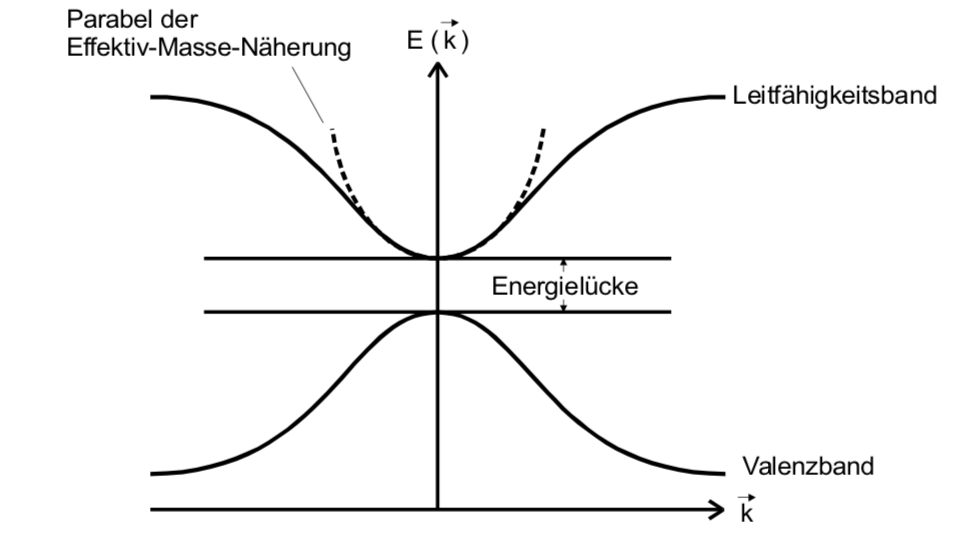
\includegraphics[height=5cm, width=8cm]{bandstruktur.png}
	\caption{Bandstruktur eines Festkörpers $^{[1]}$}   
	\label{fig: abb. 1}
\end{figure}
 Für die weitere Berechnung wird der Verlauf des Leitungsbandes näher untersucht. Für einen Wellenzahlvektor von $\vec{k}$ mit einem Minimum bei $k=0$ kann die Elektronenenergie $\epsilon$ in eine Taylorreihe entwickelt werden.
\begin{align}
\epsilon(\vec{k})=\epsilon+ \dfrac{\hbar^2k^2}{2m^{\ast}}
\end{align}
Es werden kugelförmige Energieflächen erhalten und $m^{\ast}$ stellt dabei die effektive Masse dar und beträgt
\begin{align}
m^{\ast}=\dfrac{h^2}{\left(\dfrac{\delta^2\epsilon}{\delta k_i^2}\right)_{k=0}}
\end{align}
 Diese ist deshalb vom Vorteil, weil Elektronen in einem Band wie freie Teilchen betrachtet werden können und es gilt die Quantenmechanik freier Teilchen. Beim Anlegen eines nicht zu großen äußeren elektrischen oder magnetischen Feldes kann das zweite Newtonsche Grundgesetz angewandt werden und für die weitere Berechnung des Faraday-Effektes die klassische Mechanik genutzt werden. 
\subsection{Zirkulare Doppelbrechung}
Bei der zirkularen Doppelbrechung tritt ein linear polarisierter Lichtstrahl in ein Material und ändert nach Austritt die Polarisationsebene. Zur Berechnung des Drehwinkels $\theta$ wird angenommen, dass die Lichtwelle nach Austritt des Materials in eine rechts- und linkszirkulare Welle zerlegt wird. 
\begin{align}
E(z)=\dfrac{1}{2}(E_R(z)+E_L(z))
\end{align}
Dabei sind die Phasengeschwindigkeiten von links und rechtszerkularen Anteil des Lichtes im Material unterschiedlich. Durch Umformen und Zerlegen der Gleichung (3) kann ein Ausdruck für den Drehwinkel $\theta$ ermittelt werden. 
\begin{align}
\theta= \dfrac{L\omega}{2} \left(\dfrac{1}{v_{Ph_R}}-\dfrac{1}{V_{Ph_L}}\right)
\end{align}
Mit Hilfe der Brechungsindices $n_R$ und $n_L$ wird die Gleichung (4) zu
\begin{align}
\theta= \dfrac{L\omega}{2} (n_R-n_L)
\end{align}
L ist hierbei die Länge des Materials und $\omega$ die Kreisfrequenz der einfallenden Welle. Die Doppelbrechung geschieht aufgrund des elektrischen Dipolmomentes, die durch die Atome auf den Gitterplätzen und durch die Wechselwirkung der Bandelektronen mit den Atomrümpfen erzeugt wird. Die Gesamtheit der Dipole pro Volumeneinheit, das als mikroskopische Polarisation bezeichnet wird, beträgt
\begin{align}
\vec{P}=\epsilon_0 \chi \vec{E}
\end{align}
$\chi$ ist die dielektrische Suszeptibilität. Bei isotroper Materie stellt dieser eine skalare Größe dar und bei anisotropen Kristallen einen Tensor dritter Stufe. Nach weiteren Umrechnungen erhält man für den Drehwinkel den Ausdruck 
\begin{align}
\theta= \dfrac{L\omega}{2cn}\chi_{xy    }
\end{align}
\subsection{Berechnung des Rotationswinkels $\theta$ beim Faraday Effekty}
Der Faraday Effekt und somit auch die Drehung der Polarisationsebene wird durch das Anlegen eines äußeren Magnetfeldes erzeugt. Dabei kommt es zu einer Wechselwirkung des Magnetfeldes mit den Elektronen der Materie. Für ein gebundenes Elektron gilt die folgende Bewegungsgleichung 
\begin{align}
m\dfrac{d^2\vec{r}}{d^2}+K\vec{r}=-e_0\vec{E}(r)-e_0\dfrac{d\vec{r}}{dt}\times\vec{B}
\end{align}
Dabei ist $m$ die Masse und $e_0$ die Ladung des Elektrons. Zudem steht $\vec{r}$ für die Auslenkung des Elektrons aus der Gleichgewichtslage, $K$ ist eine Konstante, die seine Bindung an die Umgebung beschreibt und $\vec{E}$ ist die Feldstärke der einfallenden Lichtwelle. Unter der Annahme, dass Dämpfungseffekte und der Einfluss des Magnetfeldes der elektromagnetischen Lichtwelle vernachlässigt werden darf, da sie nur einen geringen Einfluss auf den Faraday-Effekt haben, ergibt sich für den Winkel der Polarisationsebene mit der Proportionalität 
\begin{align}
\vec{P}=-Ne_0\vec{r}
\end{align}
und der Tensorkomponente 
\begin{align}
\chi_{xy}=\dfrac{Ne_0^3\omega B}{\epsilon_0\left(\left(-m\omega^2+K\right)^2-\left(e_0\omega B\right)^2\right)}
\end{align}
der Winkel
\begin{align}
\theta=\dfrac{e_0^3}{2\epsilon_0 c}\dfrac{1}{m^2}\dfrac{\omega^2}{\left(-\omega^2+\dfrac{K}{m}\right)^2 -\left(\dfrac{e_0}{m}B\omega\right)^2}  \dfrac{NBL}{n}
\end{align}
mit der Flussdichte $B$, der Probenlänge $L$ und der Zahl der Ladungsträger $N$ pro Volumeneinheit. $\sqrt{\dfrac{K}{m}}$ kann hier als Resonanzfrequenz $\omega_0$ und $\dfrac{Be_0}{m}$ als Zykloton-Frequenz $\omega_C$ betrachtet werden. Mittels der Annahme, dass die Messfreqenz viel kleiner als $\omega_0$ ist, lässt sich die Gleichung (11) schreiben als:
\begin{align}
\theta(\lambda)=\dfrac{2\pi^2 e_0^3 c}{\epsilon_0}\dfrac{1}{m^2}\dfrac{1}{\lambda^2 \omega_0^4}\dfrac{NBL}{n}
\end{align}
Für freie Ladungsträger ergibt sich mittels der Annahme, dass $\omega_0$ gegen Null geht:
\begin{align}
\theta_{frei}=\dfrac{e_0^3\lambda^2}{8 \pi^2 \epsilon_0 c^3 m^2 }\dfrac{NBL}{n}
\end{align}
wird $m$ durch $m^{\ast}$ ersetzt, so erhält man den Zusammenhang zwischen Drehwinkel $\theta$ und der effektiven Masse $m^{\ast}$ der Elektronen im Kristall. 
\section{Aufbau und Durchführung}
Die Abbildung (2) zeigt die schematische Darstellung der Messapparatur.  \\

\begin{figure}[H]
	\centering
	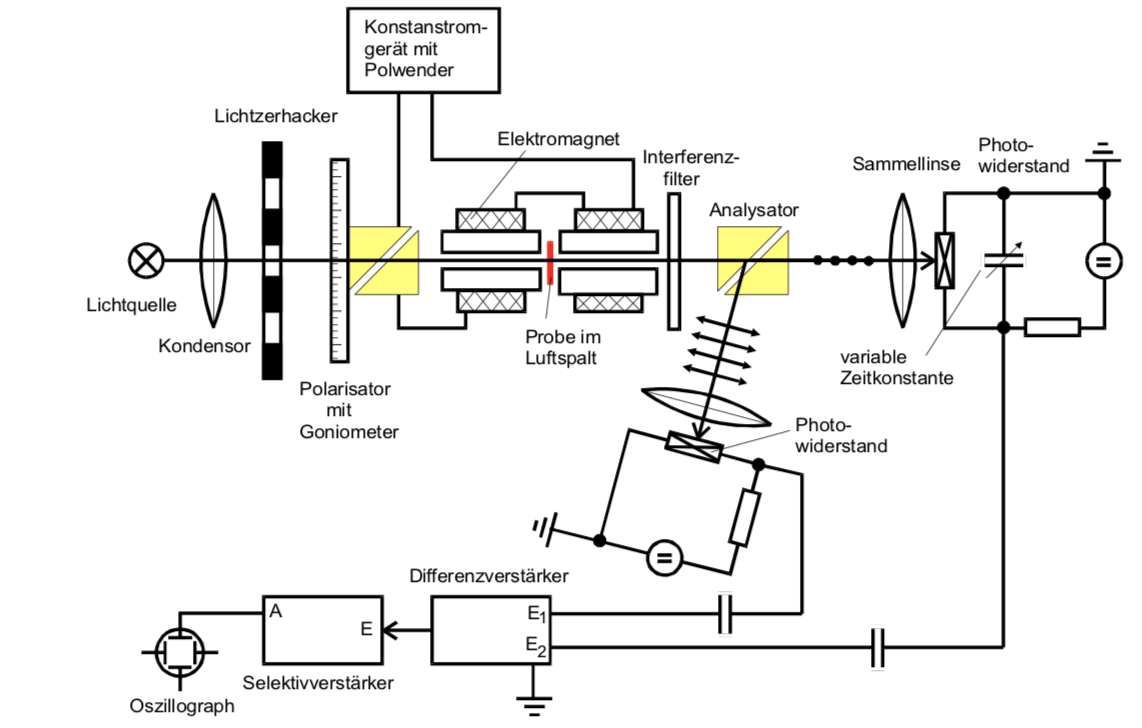
\includegraphics[height=9cm, width=12cm]{aufbau.png}
	\caption{ Versuchsapparatur $^{[1]}$}   
	\label{fig: abb. 1}
\end{figure}
Als Lichtquelle wird eine Halogen-Lampe verwendet, deren Emissionsspektrum hauptsächlich im infraroten Bereicht liegt, da die Halbleiterprobe (Galliumarsenid) nur im Infrarot durchlässig ist. Der Strahl wird mit Hilfe einer Linse gebündelt und im Lichtzerhacker, rotierende Sektorscheibe, in Lichtimpulse umgewandelt. Anschließend trifft der Strahl auf Glan-Thompson-Prisma aus Kalkspalt und wird linear polarisiert. Zur Winkelmessung dient ein Goniometer, welches zwischen dem Prisma und dem Elektromagneten angebracht ist. Im Elektromagneten befindet sich in einem Luftspalt die Halbleiterprobe. Nachdem der Lichtstrahl die Probe passiert hat, filtert der Interferenzfilter einen bestimmten Wellenlängenbereich. Anschließend trifft das monochromatische Licht auf ein zweites Glan-Thompson Prisma, welches das Licht in zwei senkrechte zueinander polarisierte Strahlen teilt. Diese werden von zwei Photowiderständen aufgenommen. Dabei wird ein Spannungssignal erzeugt, welches von der Intensität des Lichtes abhängig ist. Aufgrund des hohen Innenwidestandes in den Photowiderständen können Rauschspannungen entstehen. Deshalb wird mit der  Wechsellichtmethode gearbeitet, die durch den Lichtzerhacker gewährleistet ist. Die Wechselspannung am Photowiderstand wird mit Hilfe des Kondensators als zeitlich periodisches Licht gemessen und das Rauschen wird dabei herausgefiltert. Beide Signale der Photowiderständen werden zum Differenzverstärker geleitet. Dessen Ausgangsspannung ist proportional zur Differenz der Eingangsspannung und verschwindet dann, wenn beide Strahlen nach Betrag und Phase übereinstimmen. Anschließend wird das Ausgangssignal auf ein Selektivverstärker gegeben und am Oszilloskop, welches als Nulldetektor dient, angezeigt.\\\\
Bei der Durchführung werden die Winkel von zwei Halbleiterproben gemessen. Bei der Ersten handelt es sich um die hochreine Halbleiterprobe Galliumarsenid und bei der Zweiten um eine n-dotierte Galliumarsenid Probe (N=$1,2\cdot10{18}\text{cm}^{-3}$). Für jede Probe werden mehrere Interferenzfilter eingesetzt und die dazugehörigen Winkel gemessen.  Bei maximalem Magnetfeld kann das Prisma im Winkel verstellt und so lange variiert werden, bis der Spannungsunterschied an den Photowiderständen möglichst verschwindet. Dabei wird der erste Winkel $\theta_1$ bei dem der Spannungsunterschied am Oszilloskop verschwindet am Goniometer abgelesen. Anschließend wird das Magnetfeld umgepolt und der erste Schritt wiederholt. Der Winkel $\theta_2$ wird notiert. Der gesuchte Winkel wird mit Hilfe der Formel 
\begin{align}
\theta=\dfrac{1}{2}(\theta_1-\theta_2)
\end{align}
bestimmt. Um die Kraftflussdichte $B(z)$ entlang der Richtung des einfallenden Lichtes zu messen und die maximale Feldstärke zu bestimmen, wird eine Hallsonde im Magneten positiert und für verschiedene Positionen die Feldstärke notiert. 
\subsection{Der Interferenzfilter}
Die Abbildung (3) zeigt den schematischen Aufbau eines Interferenzfilters.
\begin{figure}[H]
	\centering
	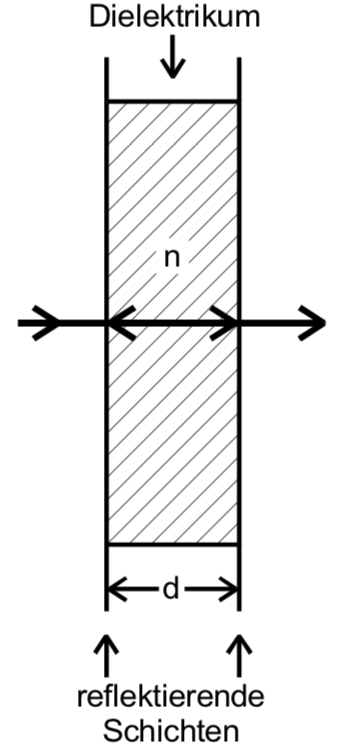
\includegraphics[height=7cm, width=3cm]{interferenz.png}
	\caption{Querschnitt durch ein Interferenzfilter $^{[1]}$}   
	\label{fig: abb. 1}
\end{figure}

 Dieser besteht aus zwei reflektierenden Schichten und dazwischen ein Dielektrikum mit der Brechnungsindex $n$. Sobald ein Lichtstrahl auf den Filter trifft, wird es an der inneren Oberfläche mehrmals reflektiert. Dabei interferieren die Teilwellen. Konstruktive Interferenz entsteht für Licht welche die Bedingung 
\begin{align}
j\lambda_j=2nd+\lambda
\end{align}
erfüllen. 
\subsection{ Das Glan-Thomson Prisma}
Die Abbildung (4) zeigt die Funktionsweise des Glan-Thomson Prismas. 
\begin{figure}[H]
	\centering
	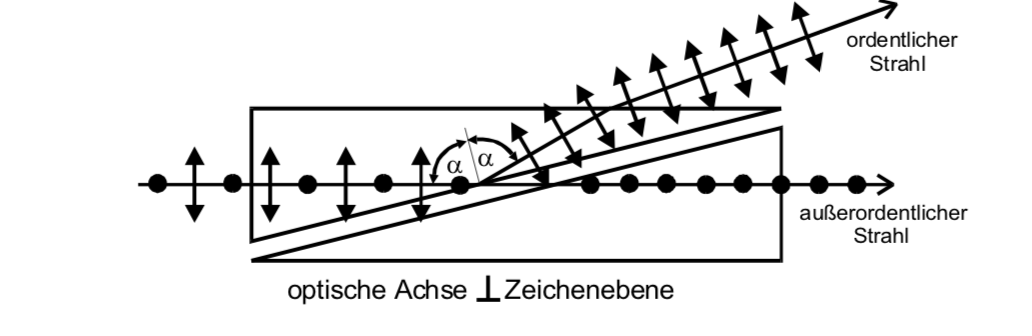
\includegraphics[height=6cm, width=14cm]{prisma.png}
	\caption{ Versuchsapparatur $^{[1]}$}   
	\label{fig: abb. 1}
\end{figure}
Es besteht aus zwei Prismen, die durch einen Luftschlitz von einander getrennt sind. Dies sorgt für eine Teilung des einfallenden Lichtstrahls in zwei senkrecht zueinander polarisierte Strahlen. Ermöglicht wird es dadurch, dass der einfallende Strahl an den Grenzflächen totalreflektiert wird, wenn das Verhältnis der Brechungsindizes 
\begin{align}
\dfrac{1}{n_0}<sin(\alpha)<\dfrac{1}{n_{ao}}
\end{align}
erfüllt ist. Hierbei ist $n_0$ der Brechungsindex des ordentlichen und $n_{ao}$ der Brechungsindex des außerordentlichen Strahls. 
	\end{document}